\documentclass[11pt]{article}
\usepackage[utf8]{inputenc}
\usepackage[T1]{fontenc}
\usepackage{lmodern}
\usepackage[a4paper,margin=2.6cm]{geometry}
\usepackage{amsmath,amssymb}
\usepackage{graphicx}
\usepackage{booktabs}
\usepackage{tabularx}
\usepackage{threeparttable}
\usepackage[font=small,labelfont=bf]{caption}
\usepackage[round,authoryear]{natbib}
\usepackage[hidelinks]{hyperref}
\usepackage{setspace}
\setstretch{1.15}
\graphicspath{{figures/}{../network-compatibility-model/figures/}{../network-compatibility-model/recipient-level/figures/}{../network-compatibility-model/identification/enigh/figures/}{../network-compatibility-model/identification/municipal-panel/figures/}}
\newcommand{\expit}{\operatorname{expit}}

\title{Migrant networks absorbed the shock: why remittances to Mexico rose during the COVID-19 pandemic}
\author{Andrea Vismara\\[2pt]\small Complexity Science Hub, Vienna, Austria \quad \texttt{vismara@csh.ac.at}}
\date{\small Draft, 29 October 2026. All numbers are generated by \texttt{network-compatibility-model/run\_all.py} in the project repository.}

\begin{document}
\maketitle

\begin{abstract}
\noindent
In April 2020 the World Bank projected that remittances to low- and middle-income countries would fall by a fifth, the sharpest decline in recent history. Remittances to Mexico, the world's second-largest recipient, instead rose: transfer counts stayed on their pre-pandemic trend in 2020 and ended 2021 about 11\% above it. We ask which mechanisms, acting through the real household--migrant networks that carry remittances, are consistent with this path and which are not. We combine the networks of 3,405 Mexican households linked to 7,999 migrants in the Mexican Migration Project with monthly US employment by occupation, and simulate household receipt month by month against Banco de M\'exico transfer counts. Job loss alone implies a 7\% drop in transfers in the second quarter of 2020. Matching the data requires near-complete replacement: when a migrant lost their job, other linked migrants made up almost all of the lost receipt. The 2021 rise is matched when more of each household's migrants send as Mexico's crisis accumulates, a response that persists into 2022. Household survey data confirm that the rise came from more transfers per receiving household rather than more receiving households, and state and municipal panels show that it was common to all regions rather than graded by local mortality. US stimulus checks shifted transfers between months without raising quarterly totals. The results reconcile survey evidence of network insurance with aggregate resilience, and suggest that forecasts built on migrant employment alone missed the capacity of networks to redistribute who sends.
\end{abstract}

\section{Introduction}

Remittances are among the largest financial flows to developing countries, larger than official aid and, for many countries, larger than foreign direct investment \citep{yang2011}. They have long been described as counter-cyclical insurance for recipient households: migrants send more when their families are hit by shocks at home \citep{lucasstark1985,yangchoi2007,bettin2017}. The COVID-19 pandemic tested this picture with a shock that hit both ends of the corridor at once. In the United States, employment among Mexican-origin workers in sales and personal services fell from 96\% to 76\% between 2019 and April 2020 \citep{ipumscps,borjascassidy2020}. In Mexico, excess mortality was among the highest recorded anywhere \citep{karlinsky2021}. Expecting migrants' earnings to collapse, the World Bank projected in April 2020 a 20\% fall in remittances to low- and middle-income countries \citep{worldbank2020brief32}.

The fall did not happen. Global remittances declined only slightly in 2020 and rose in 2021 \citep{ratha2021brief34,kpodar2023}. Mexico is the clearest case. Transfer counts recorded by the central bank \citep{banxico} were on their 2017--19 trend in 2020 (0.974 of trend in the second quarter, the trough) and about 11\% above it by the end of 2021 (Fig.~\ref{fig:puzzle}). In US dollars the rise was larger still, partly because the average transfer grew with US inflation.

Two families of explanations have been proposed. Survey and qualitative studies point to mechanisms inside migrant networks: relatives who kept their jobs stepped in for those who lost them, and migrants responded to their families' need at home \citep{garip2016,massey2002}. Macro studies explain the resilience with aggregate drivers such as US fiscal transfers, exchange rates and a shift from informal to formal channels \citep{kpodar2023}. The two literatures rarely meet. Surveys cannot say whether the mechanisms they document are large enough to explain national flows; aggregate regressions cannot say through which households the flows moved.

This paper connects the two. We build a household-level model on the actual networks that link Mexican households to US migrants, drive it with observed US job losses by occupation, and ask which combinations of mechanisms reproduce the monthly path of national transfer counts. Rather than estimating one model, we map the region of mechanism space that is compatible with the aggregate data, in the spirit of pattern-oriented modelling \citep{grimm2005}: mechanisms are retained only if they reproduce several patterns at once (the 2020 trough, the 2021 level, the 2022 out-of-sample level, and the monthly response to stimulus checks), and independent data are then used to test what the retained mechanisms imply.

Four results emerge. First, networks absorbed the employment shock. Job loss alone, passed through the real networks, implies a 7\% fall in transfers in the second quarter of 2020; the data require that other linked migrants replaced nearly all of the receipt that households would otherwise have lost. Second, the 2021--22 rise is matched by more senders per receiving household, building with the cumulative toll of the pandemic in Mexico and persisting after deaths stopped rising. Household survey data confirm that the rise was on this intensive margin, while state and municipal panels show that it was common to all regions rather than concentrated where mortality was highest. The response we find is therefore national, not local. Third, US stimulus checks moved transfers between months without raising quarterly totals, as did a rush to send at the weak peso in March 2020. Fourth, the few households that lost receipt were those with a single migrant link and nobody to step in.

The paper contributes in three ways. It provides a quantitative bridge between survey evidence on network insurance and the aggregate resilience of remittances. It shows how compatibility mapping on real network data can discriminate between mechanisms that are observationally similar in aggregate series. And it reports a well-powered negative result: the local need response often invoked to explain the 2021 surge does not appear within Mexican states, bounding it at about 0.02 log points per standard deviation of excess mortality.

\begin{figure}[t]
\centering
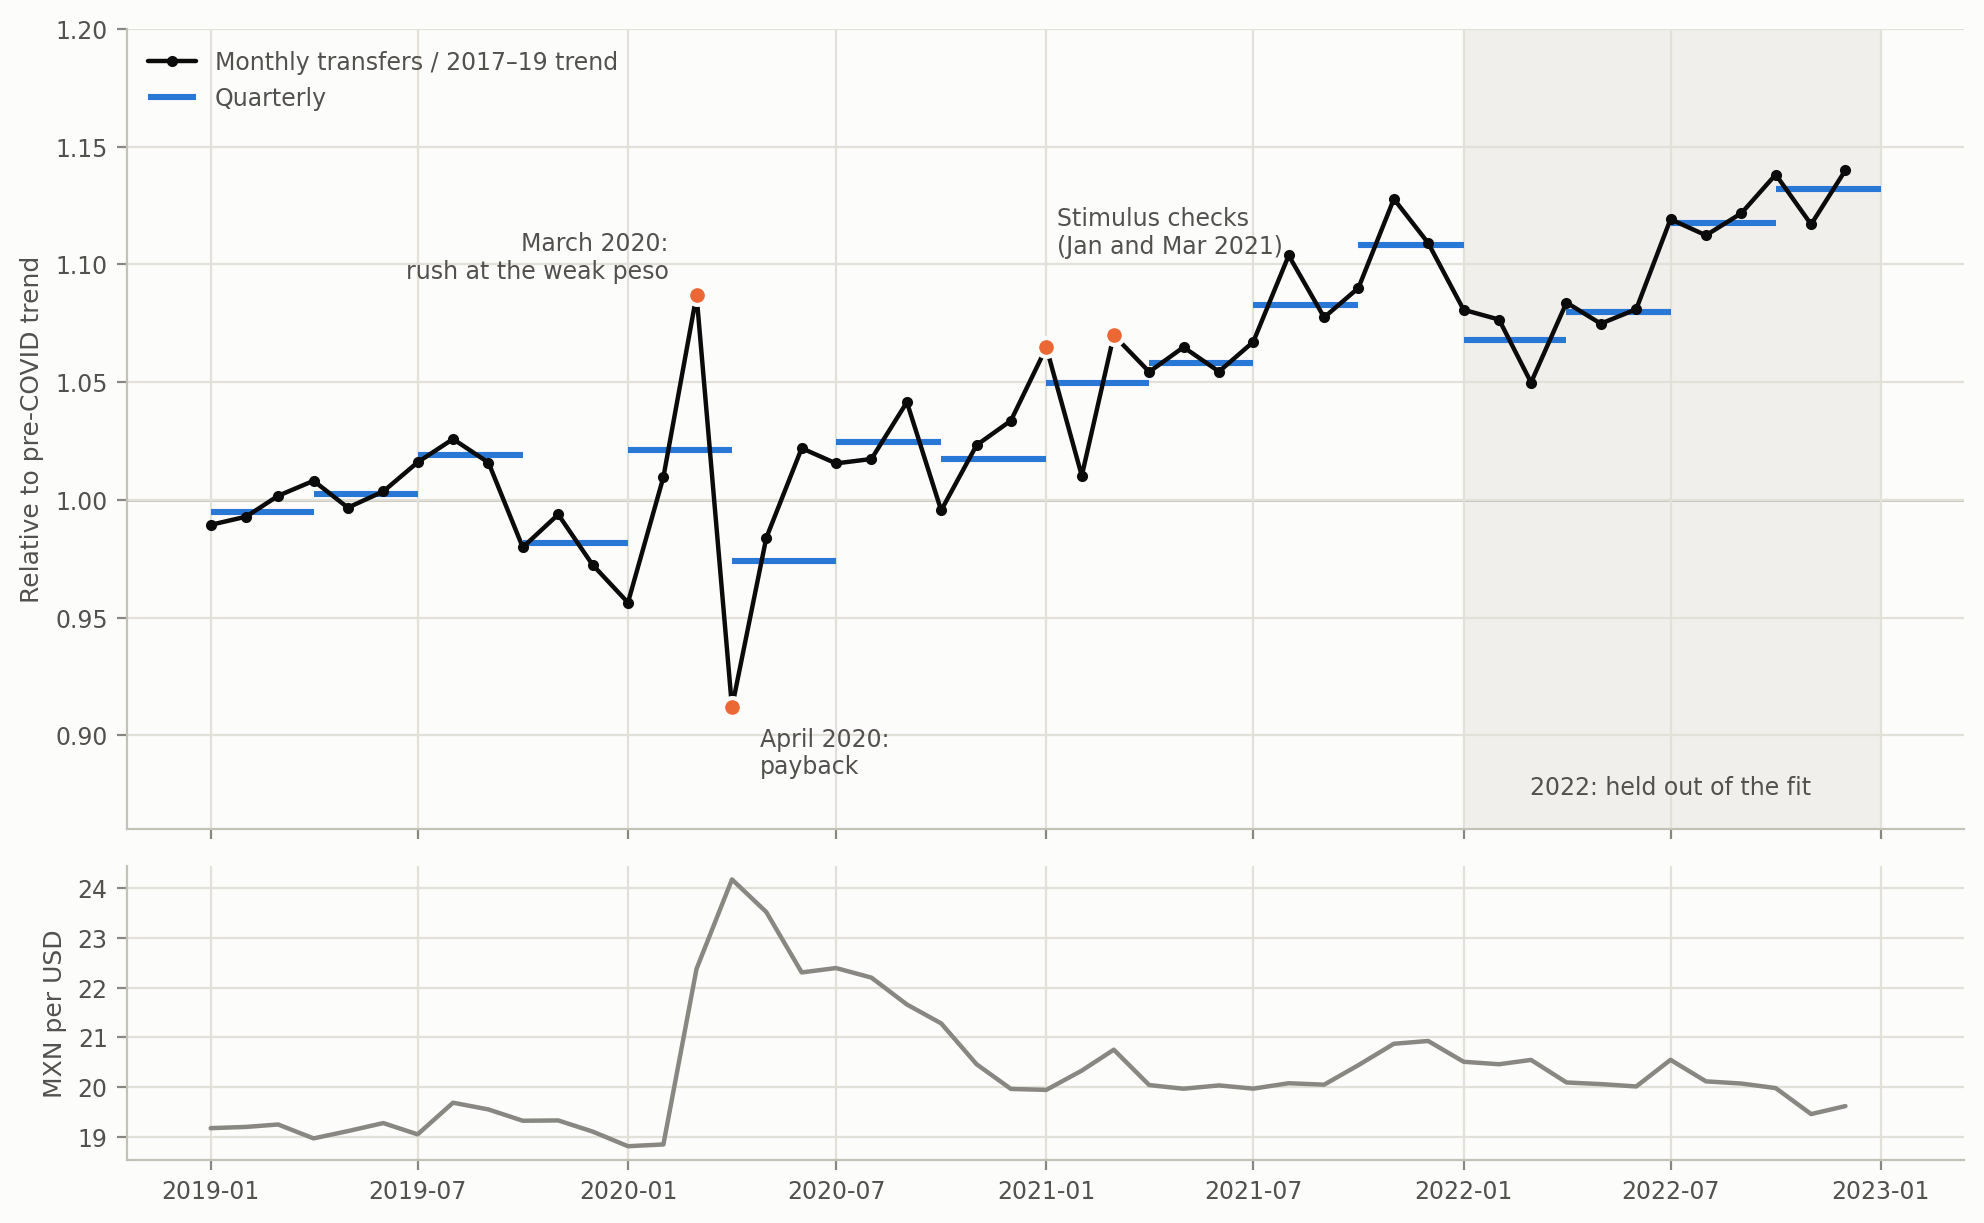
\includegraphics[width=0.92\linewidth]{F1_puzzle.png}
\caption{\textbf{Remittance transfers to Mexico did not collapse.} Top: monthly Banco de M\'exico transfer counts relative to a log-linear trend with month effects fitted on 2017--19 (+6.3\% a year), and the quarterly index (blue). Dots mark the March 2020 rush at the weak peso and the April payback (March and April together are exactly on trend, 1.000), and the US stimulus months of January and March 2021. Bottom: Mexican pesos per US dollar (monthly mean). 2022 is held out of all model fits.}
\label{fig:puzzle}
\end{figure}

\section{Results}

\subsection{The puzzle in counts}

We measure remittances by the number of transfers rather than their dollar value, because the number of transfers is closer to the behavioural margin that a household model can represent: whether, and how often, a household receives. Relative to the 2017--19 trend, transfer counts were 2.6\% below trend in the second quarter of 2020, back above it in the third quarter, 4.9\% above in the first quarter of 2021 and 10.8\% above in the fourth (Fig.~\ref{fig:puzzle}). The higher level persisted through 2022 (mean 1.10). Measured against the same quarter of 2019, counts rose by 24.4 log points by the end of 2021, of which the continuation of the pre-pandemic trend accounts for 12.3.

Two monthly features matter for interpretation. In March 2020 the peso fell sharply against the dollar (monthly means of 18.8, 22.4 and 24.2 MXN per USD in February, March and April) and transfers jumped to 1.087 of trend, before falling to 0.912 in April. Taken together, March and April were exactly on trend (1.000): migrants brought forward transfers to profit from the exchange rate, and the April trough is a payback, not a measure of the employment shock. A similar timing pattern appears around the US stimulus checks of January and March 2021, each a spike of about 4 log points above the neighbouring months. In dollars, total remittances rose by 41.6 log points to the end of 2021 against the same quarter of 2019; the extra 17.2 points over counts reflect a larger average transfer, of which US consumer-price inflation accounts for 7.8 points. The real amount per transfer was 9.4 log points higher at the end of 2021 and only 3.2 points higher at the end of 2022 (Supplementary Fig.~\ref{fig:usd}). The lasting rise is in the number of transfers.

\subsection{A household model on real migrant networks}

The model's population consists of all 3,405 households in the Mexican Migration Project's community surveys of 2010--19 \citep{mmp} that are linked to at least one migrant in the United States, 7,999 migrants in total (Fig.~\ref{fig:networks}). Each link is classified as core (the household head, spouse or a child on a US trip), close kin (parents or siblings of the head and other household members in the US) or distant kin (uncles, cousins, nephews and in-laws, aggregated into one link because receipt does not rise with their number). Most households are linked to one or two migrants, and 70\% have no core migrant at all.

In each month, every migrant is able to send if employed, with the probability of employment given by the monthly US employment rate of Mexican-origin workers in the migrant's occupation group \citep{ipumscps}. Whether a household receives in a month depends on how many of its core and kin migrants are able to send, through a logit calibrated on the households' reported receipt in 2019 employment conditions (Methods). Receipt rises steeply with having any able core migrant; kin matter only in households without a core migrant. This household-level specification fits the survey data better than a model of independent senders (Akaike information criterion 2,301 against 2,374, community-level cross-validated log loss 0.357 against 0.370).

Three behavioural mechanisms are added on top of employment. Stepping-in, $\kappa \in [0,1]$, is the share of the receipt lost to job loss that the household's other able migrants make up: $\kappa = 0$ means no replacement, $\kappa = 1$ means the household receives as long as anyone linked to it can send. Stimulus checks let migrants who are out of work send in the months the checks arrived. Need in Mexico raises each migrant's monthly probability of sending with the cumulative toll of the pandemic, measured by excess deaths; this brings additional senders into households that already receive. A count mapping translates household receipt into transfers: a household with several able senders sends several transfers (Methods). Each configuration is scored by how closely its quarterly transfer index tracks Banco de M\'exico counts relative to trend from the second quarter of 2020 to the fourth quarter of 2021, with 2022 held out.

\begin{figure}[t]
\centering
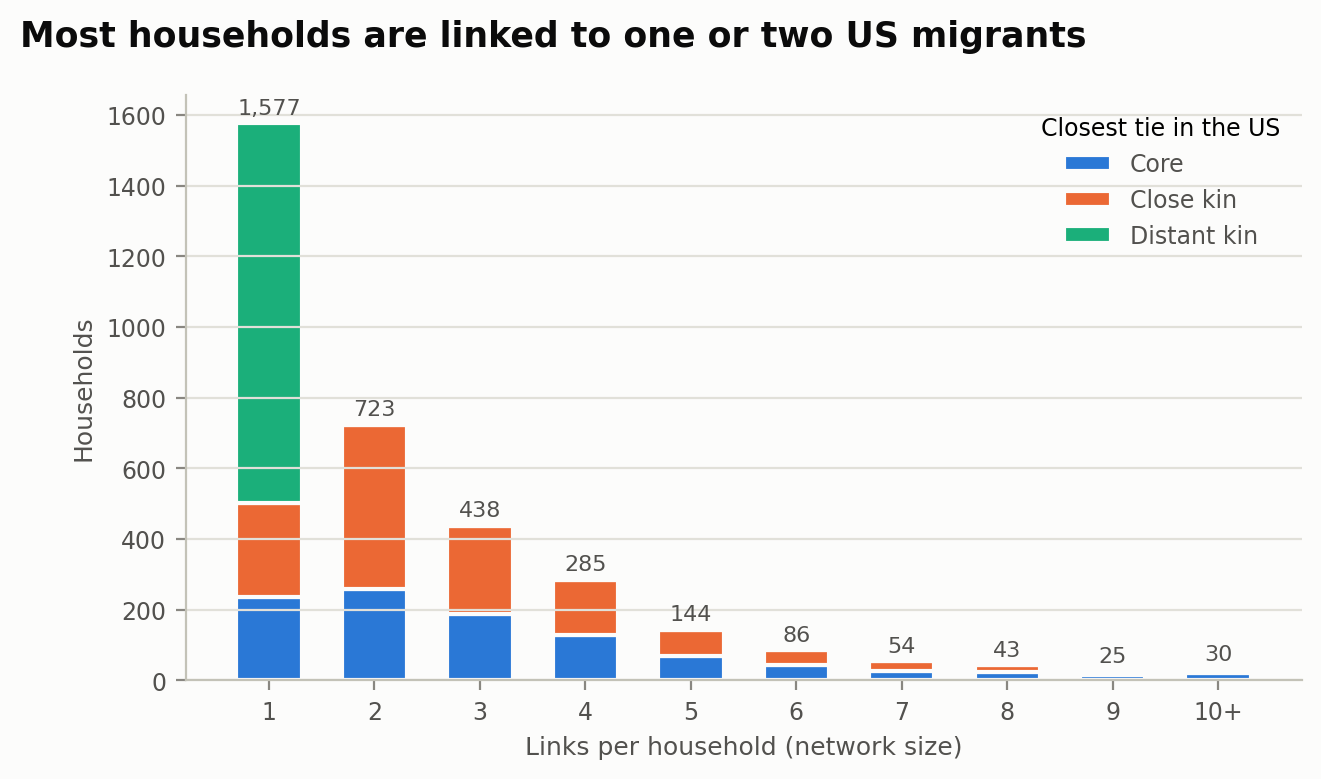
\includegraphics[width=0.85\linewidth]{A1_network_sizes.png}
\caption{\textbf{The household--migrant networks.} Number of US migrants linked to each of the 3,405 Mexican Migration Project households (2010--19 surveys), by link type. Core: head, spouse or child on a US trip; close kin: parents, siblings and other members in the US; distant kin aggregated into one link.}
\label{fig:networks}
\end{figure}

\subsection{2020: networks absorbed the employment shock}

Job loss alone produces a sharp trough. Without stepping-in, the fall in US employment passed through the real networks implies that transfers in the second quarter of 2020 were 7.0\% below their no-pandemic path (Fig.~\ref{fig:jobloss}). The data show a fall of 2.6\% relative to trend, and none at all once the March rush and April payback are pooled. Stepping-in closes most of the gap: with full replacement ($\kappa = 1$) the model's trough is 0.969 before stimulus effects or need are considered.

Across the full map of stepping-in and need (Fig.~\ref{fig:map}), the best configuration has $\kappa = 1$ and fits the quarterly path with a root-mean-square log error of 0.012, against a compatibility tolerance of 0.04 (about three times the quarterly noise of the pre-pandemic series). Its second-quarter 2020 index is 0.975, against 0.974 in the data. Two independent moments point to the same region. The 2019 survey data alone barely distinguish values of $\kappa$ (the log-likelihood varies by 1.3 points over the whole range), so the pandemic period is what identifies it. Within the pandemic, the monthly spikes around the stimulus checks are smaller when stepping-in is stronger, because the checks have less lost sending to restore; the observed spikes of +4.1 and +3.6 log points are best matched at $\kappa \approx 0.9$. Both the quarterly path and the spikes therefore imply that nearly all receipt lost to job loss was replaced by other migrants in the household's network.

\begin{figure}[t]
\centering
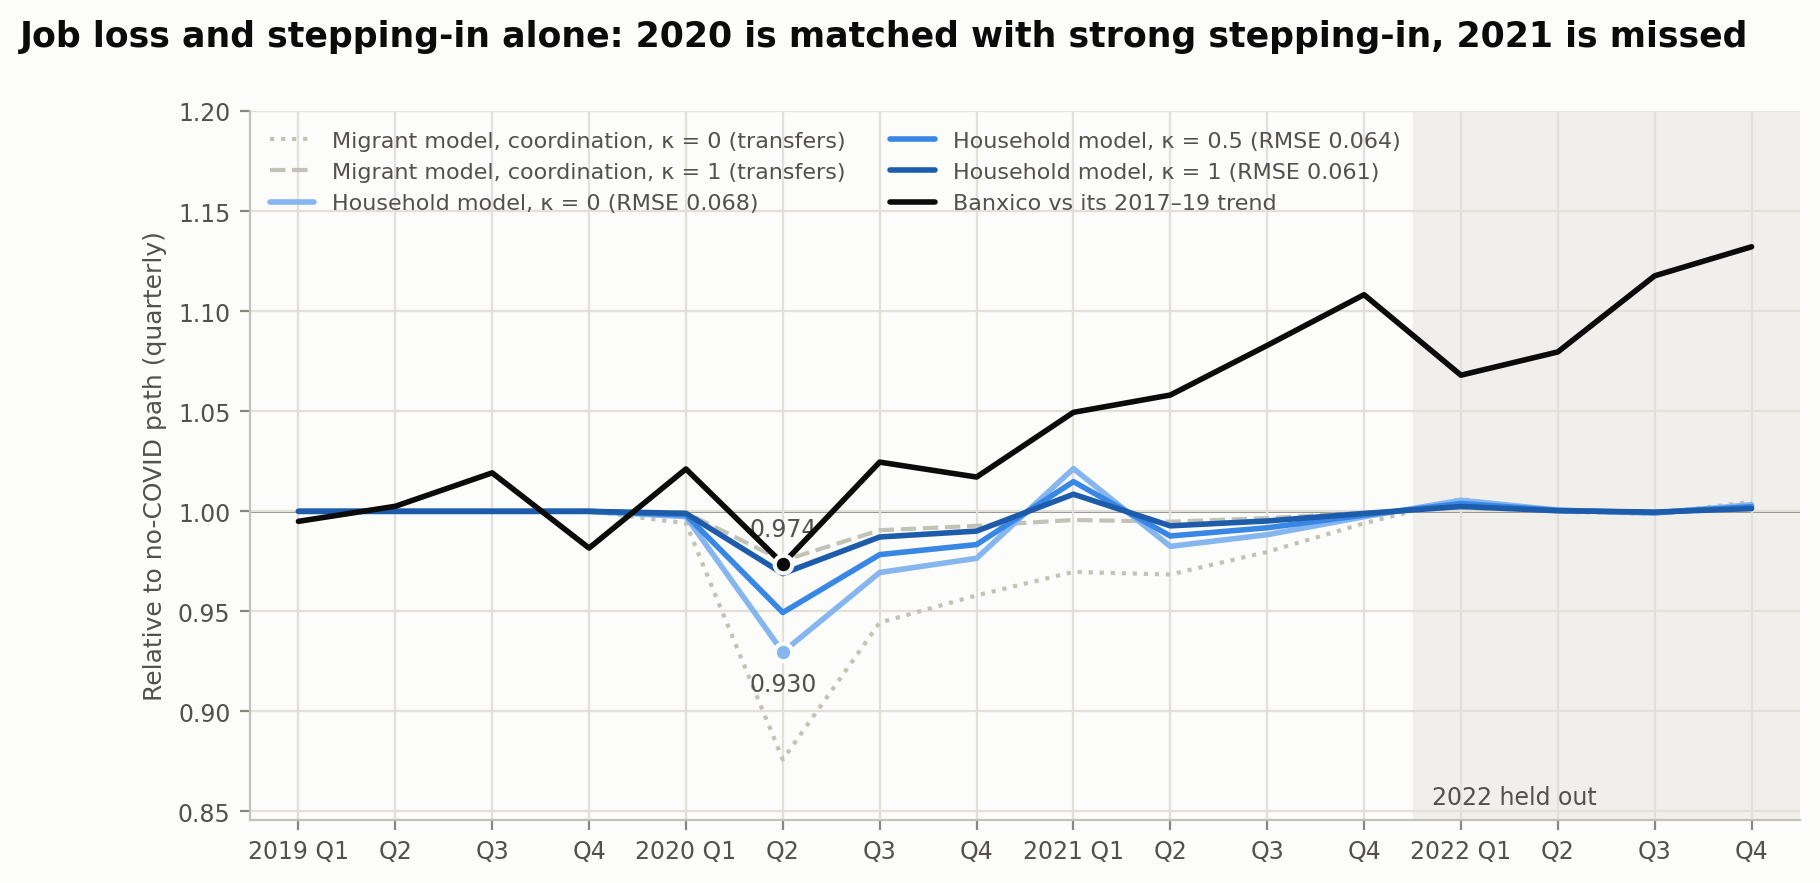
\includegraphics[width=0.92\linewidth]{S4_receipt_index.png}
\caption{\textbf{Job loss and stepping-in alone.} Household model without need ($\beta = 0$), with stimulus checks in January and March 2021, for stepping-in $\kappa$ from 0 to 1: expected receipt relative to the no-pandemic run (same calendar month of 2019 employment), quarterly, against Banco de M\'exico counts relative to trend. Gray: a migrant-level comparison model with independent senders. Without stepping-in the second quarter of 2020 falls to 0.930; with full stepping-in to 0.969. Neither configuration reproduces the 2021 rise.}
\label{fig:jobloss}
\end{figure}

\begin{figure}[t]
\centering
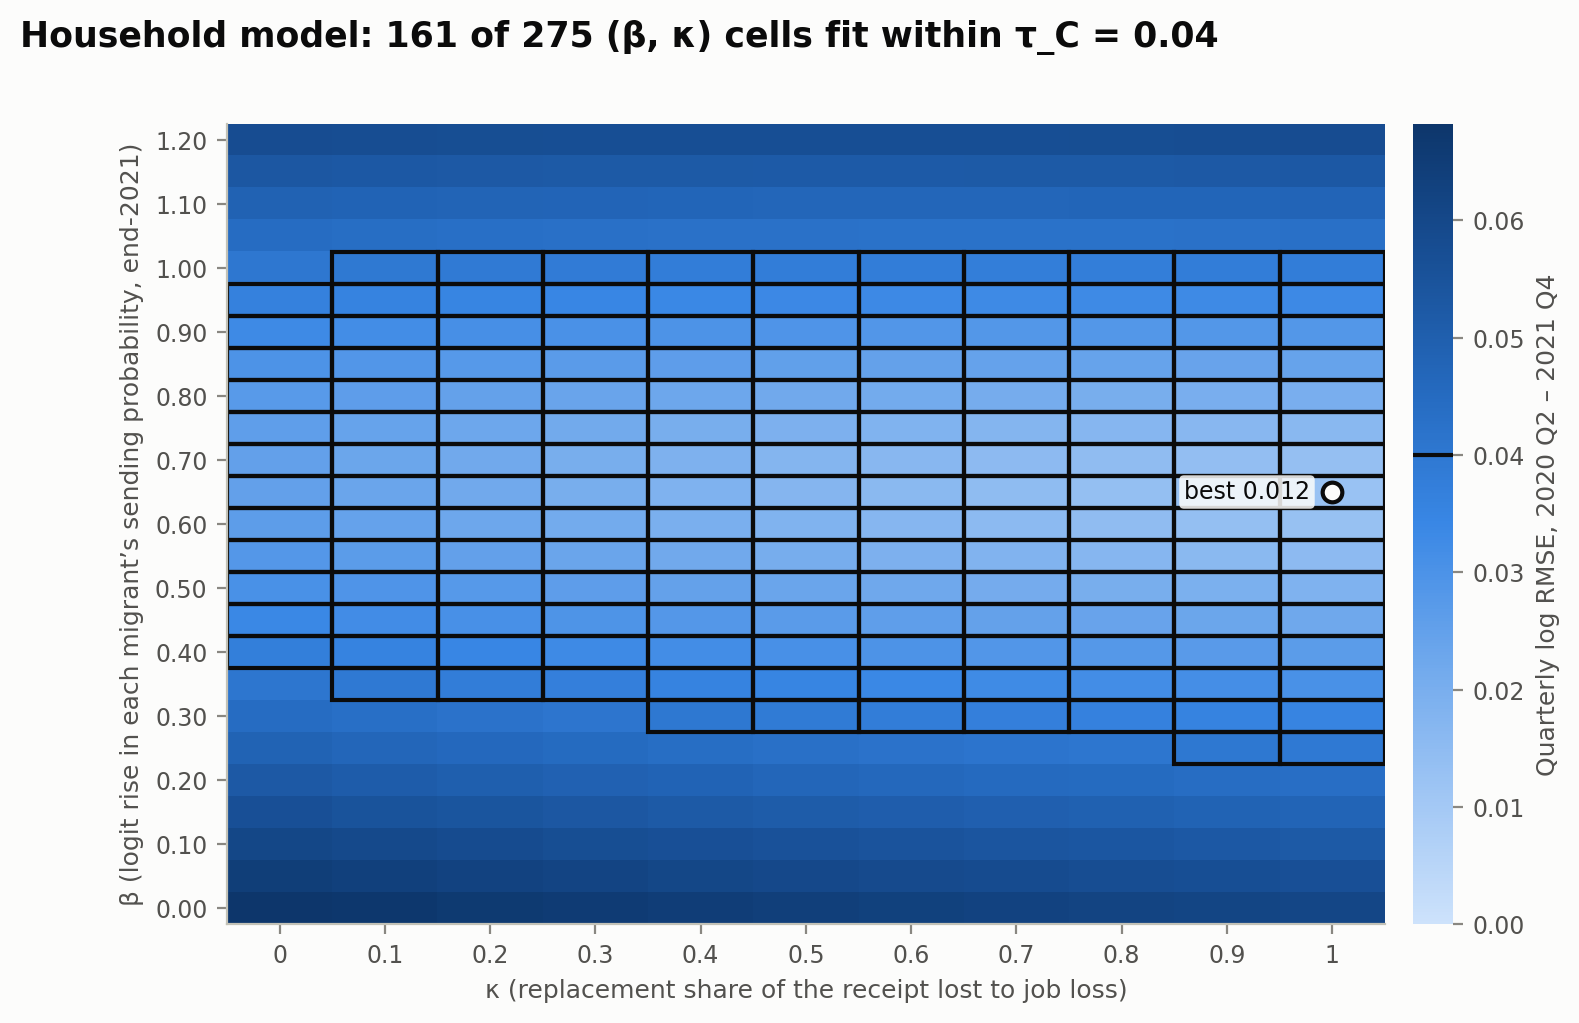
\includegraphics[width=0.78\linewidth]{S5_compatibility_map.png}
\caption{\textbf{Compatibility map.} Quarterly root-mean-square log error, 2020Q2--2021Q4, of the transfer index against Banco de M\'exico counts relative to trend, over stepping-in $\kappa$ and the need effect $\beta$ (the logit rise in every migrant's monthly sending probability at the end of 2021). Outlined: configurations within the tolerance of 0.04 (161 of 275). Dot: best configuration ($\kappa = 1$, $\beta = 0.65$, error 0.012). Receipt coefficients are refitted to 2019 for each $\kappa$.}
\label{fig:map}
\end{figure}

\subsection{2021--22: more senders as the national crisis built up}

Stepping-in cannot explain 2021. Because it can only restore receipt that job loss removed, the model with stepping-in but without need stays at its no-pandemic level through 2021 and 2022 (index 0.999 at the end of 2021), while the data rise to 1.108. The 2021 rise needs a mechanism that adds transfers beyond what migrants would have sent without the pandemic.

The mechanism we retain is that more of each household's migrants send as the crisis in Mexico accumulates. Each migrant's monthly sending probability rises with the cumulative number of excess deaths in Mexico since March 2020. Household receipt is unchanged, because the households that gain additional senders are mostly households that already receive. In the best configuration, the probability that a core migrant sends in a given month rises from 44\% in 2019 to 60\% by December 2021, and that of a kin migrant from 3.3\% to 6.2\%. This closes 86\% of the 2021 gap. Its out-of-sample error in 2022, when excess deaths stopped accumulating, is 0.024, against 0.097 without need. Decomposing the 24.4-log-point rise in counts to the end of 2021, the pre-pandemic trend contributes 12.3, job loss net of stepping-in $-0.1$, additional senders 9.1, and 3.1 remain unexplained (Fig.~\ref{fig:decomp}). The comparison model with independent senders and a need response tied to the monthly death toll leaves 10.4 points unexplained.

Three features of the time series discipline this mechanism. Persistence is essential: a need stock that decays even slowly (by 5\% a month) brings the index back down in 2022 and fails the out-of-sample test (error 0.047), and a response to the monthly flow of deaths overshoots the January 2021 spike and closes only 10\% of the gap. The choice of mortality series matters little once it is cumulated (reported COVID deaths give the same fit), whereas cumulative employment losses in Mexico, which are concentrated in 2020, fit worse. And a placebo ramp that rises linearly from March 2020 without any information on the pandemic fits as well in-sample, but keeps rising in 2022 and fails out of sample (error 0.041). What the time series identifies is therefore a response that built up through 2020--21 and stopped growing when the crisis did; the interpretation as a response to the crisis rests on the evidence that follows.

\begin{figure}[t]
\centering
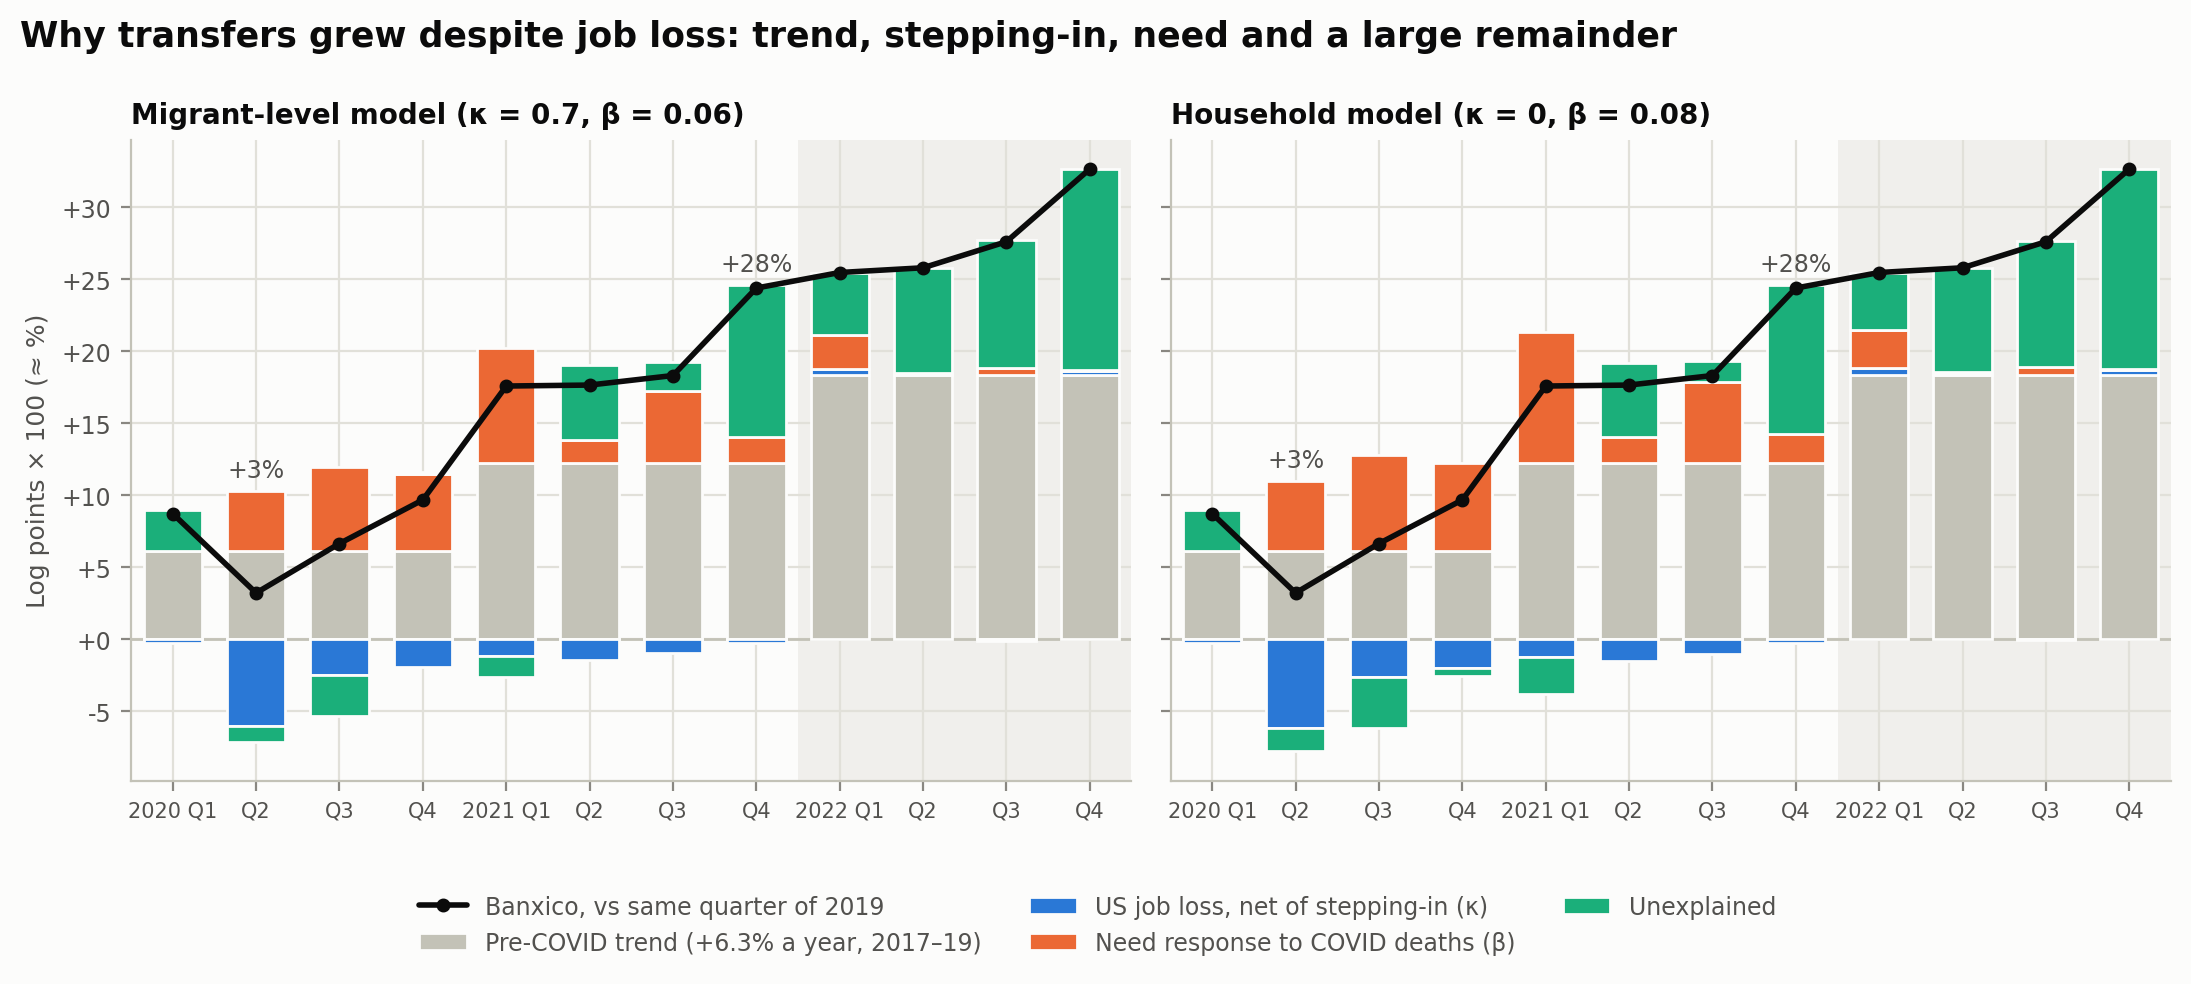
\includegraphics[width=0.98\linewidth]{S9_decomposition.png}
\caption{\textbf{Decomposition of the rise in transfer counts.} Banco de M\'exico counts relative to the same quarter of 2019 (line), split into the continued 2017--19 trend, job loss net of stepping-in, additional senders (need), and the remainder, in log points. Right: household model, best configuration ($\kappa = 1$, $\beta = 0.65$). Left: migrant-level comparison model with independent senders and a need response to the monthly death toll. 2022 held out.}
\label{fig:decomp}
\end{figure}

\paragraph{The rise was on the intensive margin.} If more senders joined households that already receive, the number of receiving households should not rise while the number of transfers does. Mexico's household income and expenditure survey \citep{enigh} allows a direct test. The share of households receiving money from abroad was 4.75\% in 2016, 4.73\% in 2018, 4.38\% in 2020 and 4.57\% in 2022. Between 2018 and 2022, Banco de M\'exico counts rose by 0.336 log points and the number of receiving households by 0.054, so transfers per receiving household rose by 0.282 (Fig.~\ref{fig:local}a). Part of this is the pre-pandemic pattern: between 2016 and 2018 transfers per receiving household already grew by 0.095 (about 4.7\% a year). Above that trend, transfers per receiving household rose by 0.09 (standard error 0.10), close to the model's 0.10 for 2022, while the number of receiving households stayed on its trend ($-0.02$, s.e.\ 0.10). The survey supports the claim that receipt did not change; it cannot pin down the size of the intensive response precisely. The survey's monthly income records also show no April 2020 dip in household receipt: the change from March to April 2020 differs from the same change in 2018 by $+0.016$ (s.e.\ 0.048).

\paragraph{The response was national, not local.} If migrants responded to their own families' need, remittances should have risen more where the crisis was worse. They did not. Across Mexico's 32 states, the 2021 deviation of remittances from each state's own 2017--19 trend is unrelated to excess mortality once pre-trends are controlled for (0.006 per standard deviation, s.e.\ 0.021; permutation $p = 0.73$). The test is sharper within states. Across 1,227 municipalities with state fixed effects and controls for pre-trends, remittance intensity, population and CONAPO's migration intensity index, the 2021 coefficient is $-0.014$ (s.e.\ 0.016, clustered by state), with a 95\% interval of $[-0.045, 0.017]$ against a mean 2021 rise of 0.14 (Fig.~\ref{fig:local}b). The median 2021 deviation is 0.178, 0.164 and 0.153 in municipalities with low, middle and high excess mortality within their state; the rise appears everywhere. An event study shows no response at the mortality peaks, and the small negative differences predate the pandemic in a 2016 placebo. Any local need response is bounded at about 0.02 log points per standard deviation of excess mortality. The rise is consistent with migrants responding to a crisis in their country of origin as a whole, through the households to which they were already sending.

\begin{figure}[t]
\centering
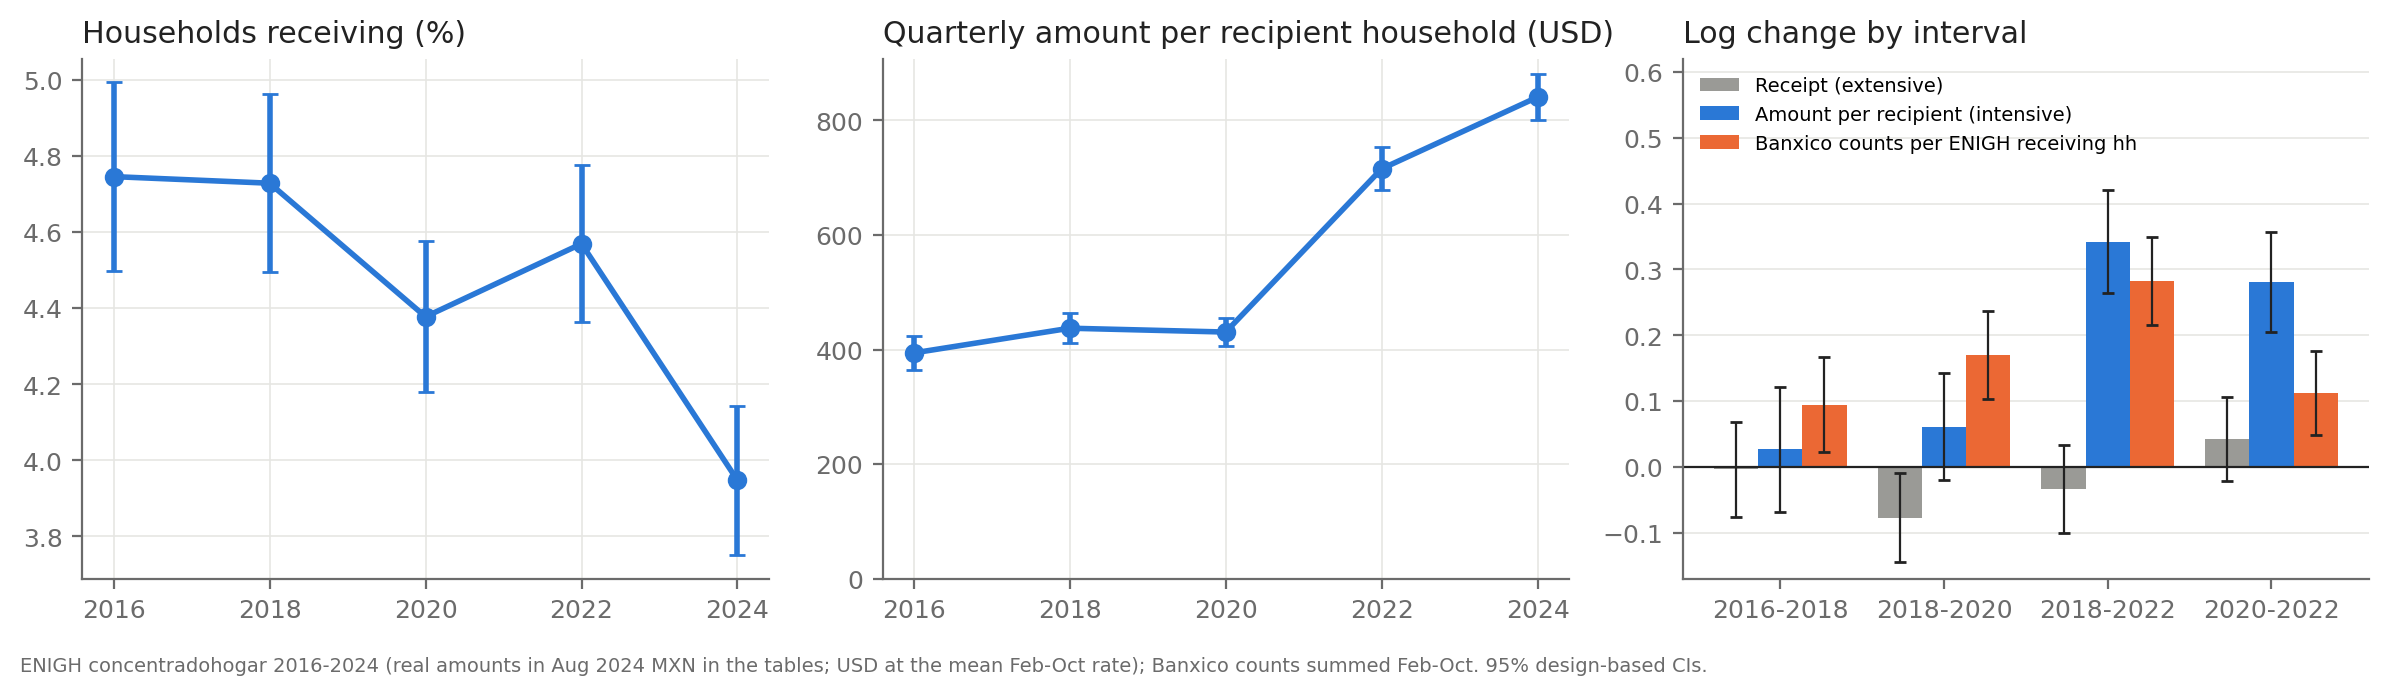
\includegraphics[width=\linewidth]{F4_pre_period.png}\\[4pt]
\small\textbf{a}\hfill\mbox{}\\[2pt]
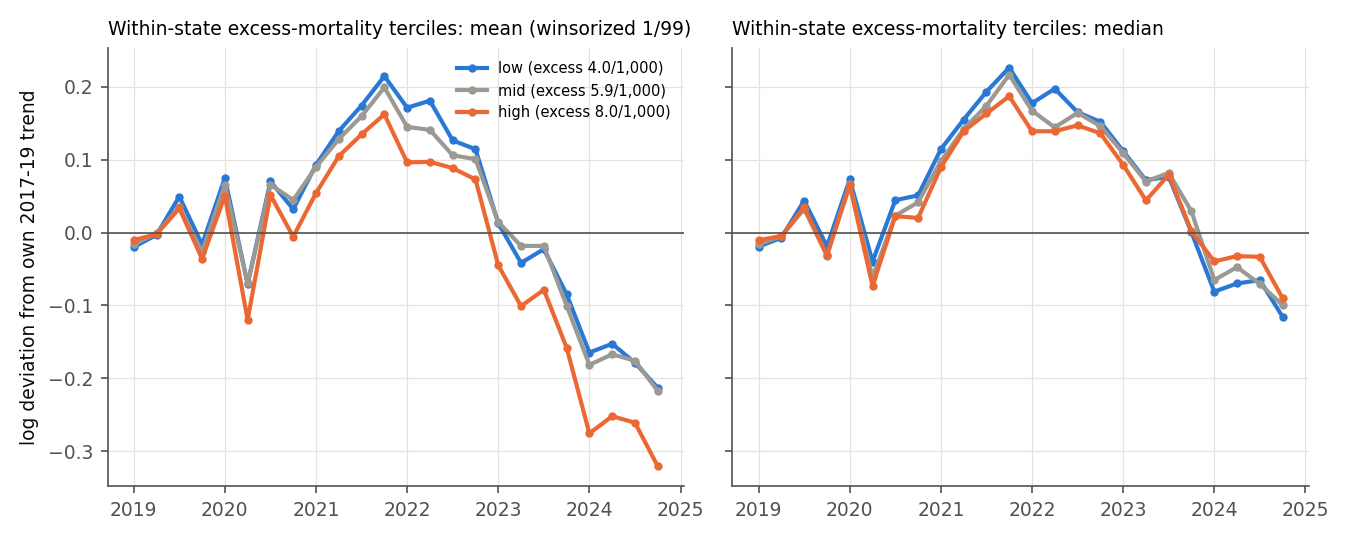
\includegraphics[width=0.92\linewidth]{F2_terciles_within_state.png}\\
\small\textbf{b}\hfill\mbox{}
\caption{\textbf{The 2021 rise was intensive and common to all regions.} \textbf{a}, Household survey (ENIGH, 2016--2024): share of households receiving money from abroad, quarterly amount per receiving household (USD), and log changes by interval in receipt (extensive), amount per recipient (intensive) and Banco de M\'exico counts per receiving household; 95\% design-based intervals. \textbf{b}, Remittances of 1,227 municipalities relative to their own 2017--19 trend, by tercile of excess mortality within their state (winsorized mean and median).}
\label{fig:local}
\end{figure}

\subsection{Stimulus checks moved transfers in time}

The model represents the stimulus checks as letting out-of-work migrants send in the months the checks arrived. With this mechanism and strong stepping-in, the model reproduces the January and March 2021 spikes (+4.1 and +2.9 log points at $\kappa = 1$, against +4.1 and +3.6). An alternative in which the checks raise every migrant's sending, whether employed or not, matches the spikes equally well; the two cannot be separated with the available data. Both, however, add transfers to the first quarter of 2021 that the quarterly data do not show: the quarterly fit is best without any stimulus effect (error 0.008 against 0.012). The spikes are compensated by lower neighbouring months, in particular February 2021, so the checks shifted when migrants sent rather than how much. The first round of checks, in April 2020, cannot be assessed from the April data because of the March payback; once March and April are pooled, letting out-of-work migrants send in April 2020 is compatible with the data. We keep the checks in the model for the spikes and treat their contribution to quarterly totals as nil.

\subsection{Who lost out}

Because stepping-in was strong, few households lost receipt. Comparing each household with its own no-pandemic twin over April 2020 to December 2021, 1.3\% of the households that would have received lost more than a quarter of their months with receipt under full stepping-in, and 0.45\% lost all of them; without stepping-in the shares would have been 3.3\% and 0.8\% (Fig.~\ref{fig:who}). Losses concentrate where there is nobody to step in: households with a single migrant link (1.1\% lost every month of receipt under full stepping-in, against none in networks of three or more) and households linked only to distant relatives (1.4\%). Households whose migrants worked in sales and personal services, the occupations hit hardest, lost most among occupational groups. The household model observes only whether a household receives; it does not capture smaller amounts within months of receipt.

\begin{figure}[t]
\centering
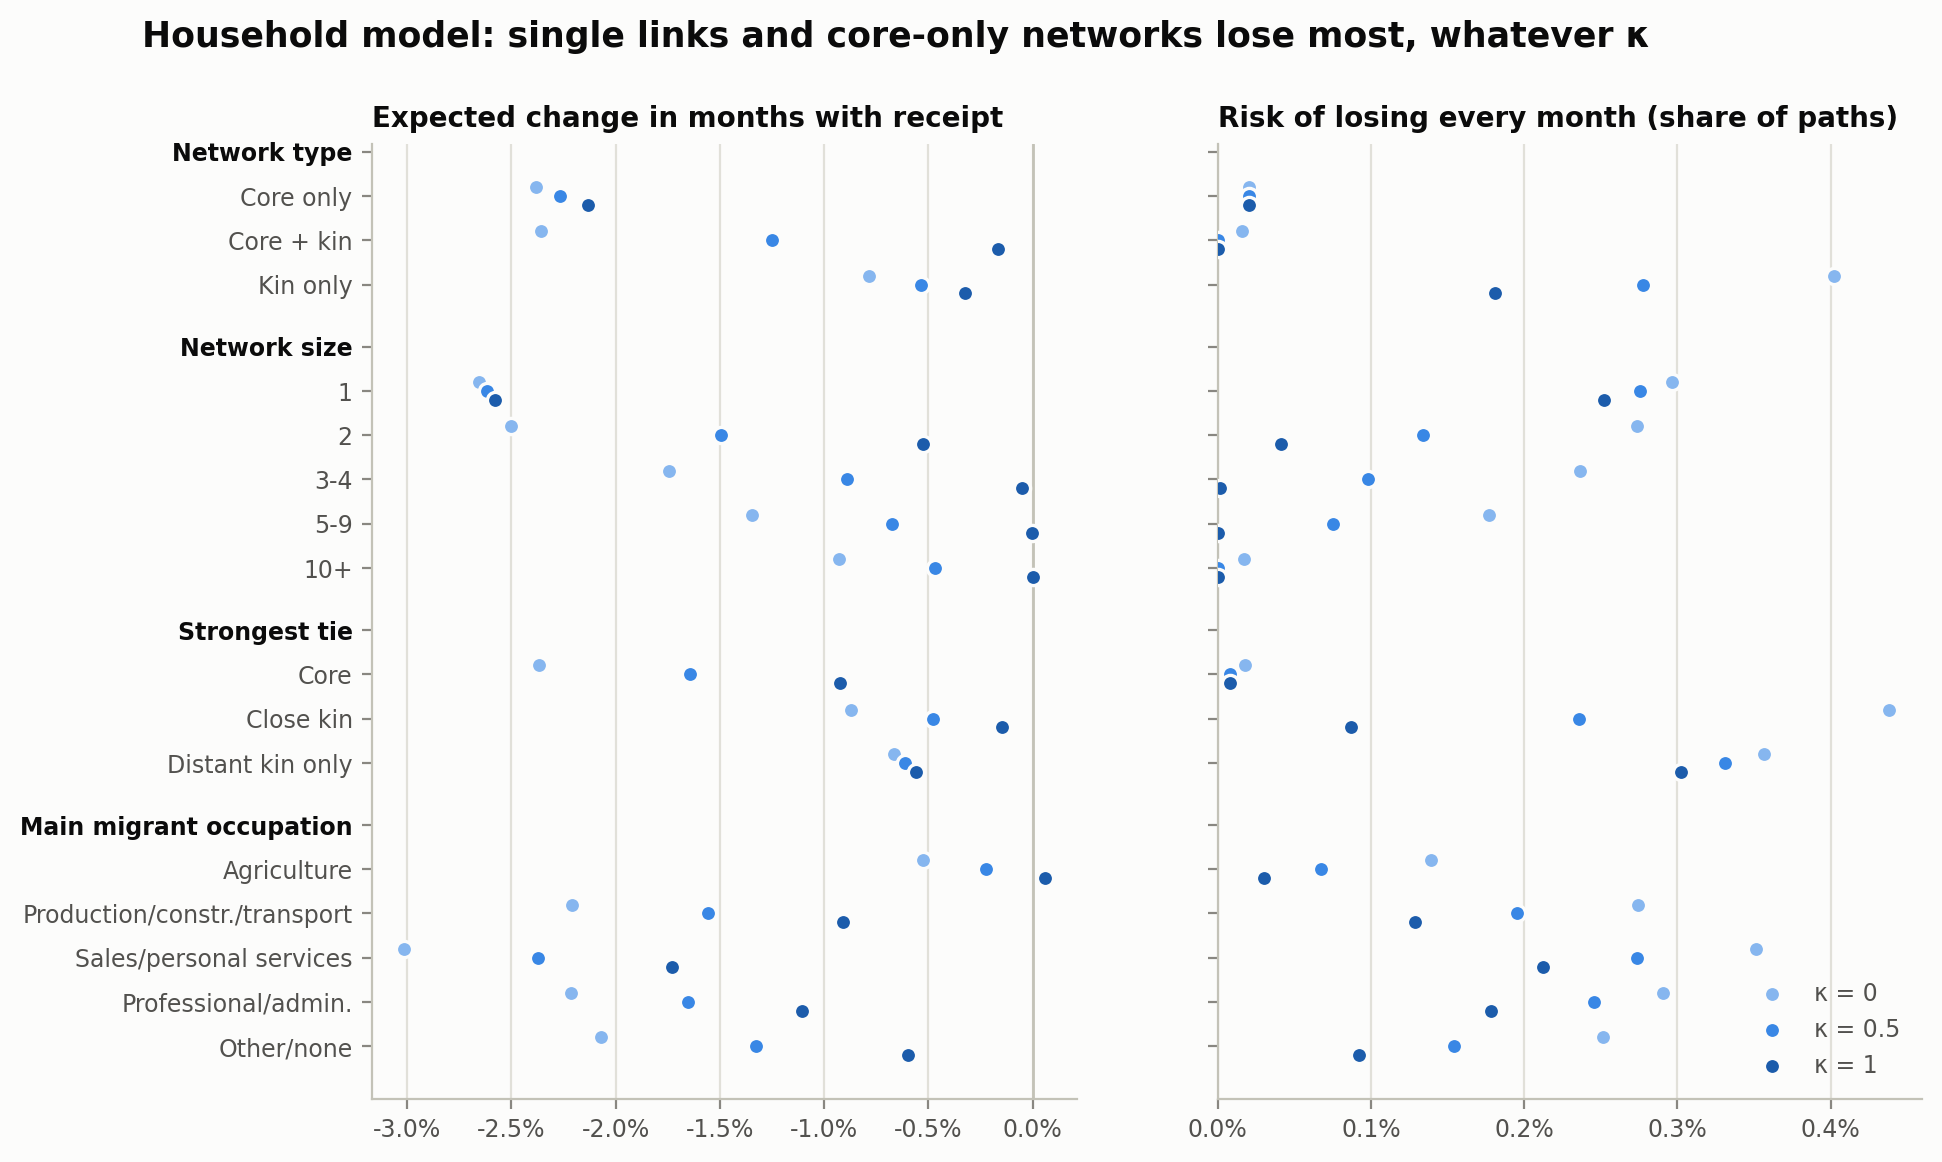
\includegraphics[width=0.95\linewidth]{S8_who_loses.png}
\caption{\textbf{Who lost out.} Left: expected change in months with receipt, April 2020--December 2021, against each household's no-pandemic twin, by network type, size, strongest tie and main migrant occupation, for $\kappa = 0, 0.5, 1$. Right: share of paths in which a household that receives in its no-pandemic twin receives in no month. 200 paired simulations with common random numbers.}
\label{fig:who}
\end{figure}

\subsection{Robustness}

Table~\ref{tab:robust} summarizes eight robustness analyses; each first reproduces the base results exactly. Stepping-in near full replacement, the 2020 trough, the 2021--22 level and the small remainder are robust to all of them. Allowing out-of-work migrants to send from savings substitutes for stepping-in (the best $\kappa$ falls to 0.5 if they send with half their usual probability), but makes the 2020 trough too shallow and the stimulus spikes too small, so the data favour small savings effects. The count mapping matters for 2020: if a relative who steps in restores receipt but not all lost transfers, the trough deepens to 0.945 and the spikes double; the data tolerate at most a quarter of transfers being lost in this way. In normal times the model is inert: calibrated on 2018 employment and run forward through 2019, its index stays within $\pm 0.5\%$ per quarter. The size of the need effect is the most assumption-dependent quantity: depending on the window used for the pre-pandemic trend, the end-2021 rise in a core migrant's sending probability ranges from 14 to 22 percentage points, and the remainder from +0.5 to +4.2 log points.

\begin{table}[t]
\centering
\small
\begin{threeparttable}
\caption{\textbf{Robustness.} Household model at $\kappa = 1$ with $\beta$ refitted; ``best $\kappa$'' minimizes the quarterly error. Data: 2020Q2 0.974, 2021Q4 1.108, spikes +4.1 / +3.6.}
\label{tab:robust}
\begin{tabular}{lcccccc}
\toprule
Variant & best $\kappa$ & $\beta$ & Error & 2022 error & 2020Q2 & Spikes \\
\midrule
Base & 1.0 & 0.64 & 0.012 & 0.024 & 0.975 & 4.1 / 2.9 \\
\addlinespace
Savings, 25\% & 0.9 & 0.63 & 0.012 & 0.023 & 0.984 & 3.0 / 2.1 \\
Savings, 50\% & 0.5 & 0.61 & 0.013 & 0.023 & 0.992 & 2.1 / 1.4 \\
Stimulus in April 2020 ($\pi = 1$) & 1.0 & 0.64 & 0.014 & 0.024 & 0.991 & 4.1 / 2.9 \\
Stimulus raises all sending ($\gamma$) & 0.9 & 0.64 & 0.013 & 0.024 & 0.975 & 4.1 / 3.6 \\
No stimulus effect & 1.0 & 0.67 & 0.008 & 0.025 & 0.975 & 1.2 / 0.6 \\
March and April 2020 pooled\tnote{a} & 1.0 & 0.65 & 0.016 & 0.024 & 0.975 & 4.1 / 2.9 \\
\addlinespace
Need: reported COVID deaths & 1.0 & 0.65 & 0.012 & 0.024 & 0.974 & 3.9 / 2.9 \\
Need: employment loss in Mexico & 1.0 & 0.47 & 0.023 & 0.037 & 0.990 & 3.8 / 2.9 \\
Need decays 5\% a month & 1.0 & 0.56 & 0.018 & 0.047 & 0.977 & 4.3 / 3.0 \\
Need as monthly flow & 1.0 & 0.82 & 0.046 & 0.093 & 1.000 & 10.4 / 1.5 \\
Kin senders only & 1.0 & 1.87 & 0.011 & 0.033 & 0.972 & 4.0 / 2.9 \\
Placebo ramp & 1.0 & 0.71 & 0.009 & 0.041 & 0.980 & 3.6 / 2.8 \\
\addlinespace
Lost transfers despite stepping-in, 25\% & 1.0 & 0.60 & 0.014 & 0.024 & 0.965 & 5.1 / 3.7 \\
Lost transfers despite stepping-in, 100\% & 1.0 & 0.52 & 0.021 & 0.026 & 0.945 & 7.3 / 5.5 \\
\addlinespace
Trend 2015--19 & 1.0 & 0.50 & 0.015 & 0.026 & 0.973 & 3.9 / 2.8 \\
Trend 2010--19 & 1.0 & 0.88 & 0.020 & 0.038 & 0.977 & 4.4 / 3.1 \\
\bottomrule
\end{tabular}
\begin{tablenotes}\footnotesize
\item[a] Error on eight periods with March--April and May--June 2020 pooled.
\item Error: quarterly root-mean-square log error 2020Q2--2021Q4; 2022 error: same over 2022 (held out). Spikes: January and March 2021, log points over the mean of neighbouring months. Out of sample (calibrate on 2018 employment, run 2019): quarterly deviation from 1 of 0.001--0.003. Full results: \texttt{outputs/robustness/summary.csv}.
\end{tablenotes}
\end{threeparttable}
\end{table}

\section{Discussion}

Forecasts of a remittance collapse in 2020 were built on a simple chain: migrants lose jobs, migrants send less. The chain was correct in its first link and wrong in its second. Mexican-origin employment in the United States fell sharply, and passed through the real household--migrant networks it implies a fall of 7\% in transfers at the trough. The fall did not materialize because networks redistributed who sent. When one migrant lost their job, another linked to the same household kept or took over the sending. This is the insurance function of migrant networks documented in survey work \citep{garip2016,massey2002,munshi2003}, operating at a scale that offset most of one of the largest employment shocks the corridor has seen.

The 2021 surge requires a second mechanism, and the evidence points to a specific form. More migrants sent to households that were already receiving, as the crisis in Mexico accumulated. The response was persistent, consistent with sending habits that, once formed, continued after deaths stopped rising. It was national rather than local: within Mexican states, municipalities with higher excess mortality saw no larger rise. This refines the standard account of remittances as insurance against shocks at home \citep{yangchoi2007,bettin2017}. The insurance motive may have been triggered by a shared sense of crisis in the country of origin rather than by the specific losses of each family, or the households hit hardest may not have been the ones with the strongest links abroad. Either way, models that tie remittance responses to local shocks would have predicted a geographic pattern that the data do not show.

The stimulus checks are a smaller part of the story than often suggested. They are visible as monthly spikes but leave quarterly totals unchanged, and the first round in April 2020 is confounded by the exchange-rate rush in March. Policies that change when migrants can send therefore move monthly flows without necessarily changing what households receive over a quarter. The March 2020 episode is itself informative: migrants responded within days to a depreciation of the peso of about 20\%, which suggests that a share of transfers is timed opportunistically and that monthly remittance series contain substantial timing noise around policy and exchange-rate events.

The approach has wider use. Many questions about how social networks transmit or absorb shocks cannot be answered by aggregate regressions, which do not see the networks, or by surveys, which do not see the aggregate. A model built on observed networks, driven by observed shocks and constrained by several aggregate patterns at once, can separate mechanisms that are indistinguishable in either source alone. Here, stepping-in and need responses produce similar annual totals but different troughs, different responses to stimulus checks and different implications for household surveys and regional panels.

\paragraph{Limitations.} The model observes household receipt, not amounts, and maps receipt to transfer counts through the expected number of senders per receiving household. The network data come from community surveys conducted before the pandemic, concentrated in traditional sending regions, and the migrant links are those reported by origin households. The model's monthly receipt probability is calibrated to households' reported receipt, which is a mapping assumption. Need is interpreted, not identified: the time series supports a response that builds up and persists, and the cross-sectional evidence locates it on the intensive margin and at the national level, but alternative drivers with the same shape, such as rising US wages or a shift towards recorded channels, cannot be excluded. The size of the need effect depends on the assumed pre-pandemic trend. The model leaves a level gap of about two log points in early 2020, which savings or the first stimulus round could fill.

\section{Methods}

\subsection{Data}

\paragraph{Remittances.} Monthly number of remittance transactions and total value in US dollars, 2013--2025 \citep{banxico}. The target is the number of transactions relative to a log-linear trend with month effects fitted on January 2017 to December 2019 (+6.3\% a year), aggregated to quarters. The quarterly residual standard deviation of the trend fit in 2017--19 is 0.014. State and municipal remittances in US dollars come from Banco de M\'exico table CE166 (2013--2026, quarterly); transaction counts are not published below the national level.

\paragraph{Networks.} All households in the Mexican community surveys of the Mexican Migration Project interviewed in 2010--19 that are linked to at least one migrant currently in the United States \citep{mmp}: 3,405 households in 46 communities and 7,999 migrant links. Core migrants are the household head, spouse or children on a US trip at the time of the survey; close kin are the head's parents and siblings and any other member in the United States; distant relatives (uncles and aunts, cousins, nephews and nieces, in-laws) are aggregated into one link per household, because household receipt rises with close kin but not with the number of distant relatives. Each migrant's occupation is that of the last US trip, grouped into agriculture; production, construction and transport; sales and personal services; and professional and administrative work. Migrants coded as not working on the last trip are assigned the all-occupation employment rate. The calibration sample consists of the 3,252 households with complete records and known receipt, of which 756 (23.2\%) report receiving remittances. Household need features are whether the household has no resident worker and whether it has a resident aged 65 or older.

\paragraph{Employment.} Monthly employment rates (employed over employed plus unemployed, by occupation of current or last job) for workers of Mexican origin aged 18--64 in the Current Population Survey, 2017--2023 \citep{ipumscps}, smoothed over three months only where cells are small. The extract does not identify birthplace, so Mexican origin is used. Month-to-month persistence of individual employment ($\phi = 0.91$) is estimated from linked CPS records.

\paragraph{Need and stimulus.} Monthly excess deaths in Mexico against a trend baseline from the World Mortality Dataset \citep{karlinsky2021}, with negative months set to zero. The stimulus months are April 2020, January 2021 and March 2021.

\paragraph{Household surveys and regional panels.} ENIGH 2016--2024 \citep{enigh}: receipt is any income from abroad in the household summary table; amounts are deflated to August 2024 pesos and converted to dollars at the mean February--October exchange rate; standard errors are design-based (primary sampling units, strata and weights). Monthly receipt uses the six monthly amounts of the person-level income table (code P041, which sums exactly to the household total). State and municipal excess mortality is computed from death certificates by place of residence against the 2015--19 average.

\subsection{Model}

\paragraph{Ability to send.} Migrant $j$ with occupation $o(j)$ is able to send in month $t$ with probability $e_{o(j),t} + (1 - e_{o(j),t})\,\pi_t$, where $e$ is the CPS employment rate and $\pi_t = 1$ in January and March 2021 (stimulus checks; second and third rounds, which included more mixed-status families) and 0 otherwise, including April 2020. Abilities are independent across migrants given the rates, so the numbers of able core and kin migrants of household $h$, $A^c_{h,t}$ and $A^k_{h,t}$, follow Poisson-binomial distributions computed exactly.

\paragraph{Receipt.} With $a$ able core and $b$ able kin migrants, household $h$ receives with probability
\begin{equation}
s_h(a,b) = \expit\big(b_0 + b_{\mathrm{any}}[a > 0] + b_c \log(1+a) + b_k \log(1+b) + b_{k0}[N^c_h = 0]\log(1+b) + \eta' x_h\big),
\end{equation}
where $N^c_h$ is the household's number of core migrants and $x_h$ the need features. Stepping-in adds a share $\kappa$ of the receipt lost to job loss whenever at least one linked migrant can send:
\begin{equation}
P_{h,t} = \mathbb{E}\Big[s_h(A^c_{h,t}, A^k_{h,t}) + \kappa\,[A^c_{h,t} + A^k_{h,t} > 0]\big(s_h(N^c_h, N^k_h) - s_h(A^c_{h,t}, A^k_{h,t})\big)\Big].
\end{equation}
For each $\kappa \in \{0, 0.1, \dots, 1\}$ the seven coefficients are estimated by maximum likelihood on the households' reported receipt under 2019 employment rates. At $\kappa = 1$: $b_0 = -3.93$ (s.e.\ 0.23), $b_{\mathrm{any}} = 4.04$ (0.31), $b_c = 0.51$ (0.20), $b_k = -0.16$ (0.12), $b_{k0} = 1.30$ (0.22), no resident worker 0.38 (0.15), older resident 0.22 (0.13). The model's mean monthly receipt probability is matched to the share of households reporting receipt.

\paragraph{Need and transfer counts.} Each migrant sends in a month with probability $\theta_{j,t} = \expit(\alpha_j + \beta N^*_t)$, with $\alpha_{\mathrm{core}} = -0.23$ and $\alpha_{\mathrm{kin}} = -3.37$ estimated by maximum likelihood in a migrant-level model of the same survey data, and $N^*_t$ the cumulative excess deaths since March 2020 scaled to 1 in December 2021 ($N^* = 0$ before the pandemic and in the counterfactual). The expected number of able senders in a receiving household is $r_{h,t}(\beta) = \sum_j q_{j,t} / (1 - \prod_j (1 - q_{j,t}))$ with $q_{j,t} = (\text{ability}) \times \theta_{j,t}$. Transfers are $\sum_h P_{h,t}\, r_{h,t}(\beta)/r_{h,t}(0)$: transfers per receiving household are constant except for the senders that need brings in. A lower-bound mapping, $\sum_h P_{h,t}\, r_{h,t}(\beta)$, lets job loss reduce transfers within receiving households even when stepping-in restores receipt; mixtures of the two are reported in the robustness analysis.

\paragraph{Index, fit and compatibility.} The model index is the ratio of expected transfers in the pandemic run to those of a counterfactual run with the employment rates of the same calendar month of 2019 and no need. It is compared quarterly with Banco de M\'exico counts relative to trend; the fit criterion is the root-mean-square log error over 2020Q2--2021Q4 (seven quarters), a configuration is compatible if this is at most 0.04, and 2022 is held out. The map covers $\kappa \in [0,1]$ in steps of 0.1 and $\beta \in [0, 1.2]$ in steps of 0.05; $\beta$ is also fitted continuously for each $\kappa$. Stimulus spikes are the log monthly index in January and March 2021 minus the mean of the log index in the neighbouring months.

\paragraph{Household outcomes.} Two hundred paired simulations draw individual employment from a latent Gaussian autoregressive process matching the CPS rates and persistence, with common random numbers for employment and receipt in the pandemic and counterfactual runs. Outcomes are the change in months with receipt, April 2020--December 2021, of each household against its counterfactual twin.

\paragraph{Comparison model.} A migrant-level model in which each able migrant sends independently with probability $\theta_j$, with stepping-in as a proportional rise in the sending of the household's able migrants and need as a response to the monthly death toll, is fitted to the same data. It fits the 2019 survey worse (Akaike information criterion 2,374 against 2,301 for the household logit without the kin--no-core term) and the pandemic path worse (best error 0.043, outside the tolerance; 2022 error 0.091).

\paragraph{Regional panels.} For each state and municipality, the outcome is the log deviation of annual remittances from its own 2017--19 log-linear quarterly trend with quarter effects. Excess mortality is standardized. State regressions use heteroskedasticity-robust standard errors and permutation tests; municipal regressions include state fixed effects, the pre-trend slope, log remittances per capita in 2019, log population and the 2020 municipal migration intensity index, with standard errors clustered by state. The municipal sample contains the 1,227 municipalities with positive remittances in every quarter of 2017--19 and at least USD 1 million in 2019, covering 99.5\% of remittances; 100\% of Banco de M\'exico municipality names were matched to census codes. The minimum detectable effect at 80\% power is 0.045 log points per standard deviation.

\subsection{Data and code availability}

All code is available in the project repository; a single script rebuilds every result. Mexican Migration Project and IPUMS CPS microdata are available from their providers under their terms and are not redistributed; all other inputs are public. Outputs are aggregates.

\bibliographystyle{plainnat}
\bibliography{refs}

\clearpage
\appendix
\renewcommand{\thefigure}{S\arabic{figure}}
\setcounter{figure}{0}
\section*{Supplementary figures}

\begin{figure}[h]
\centering
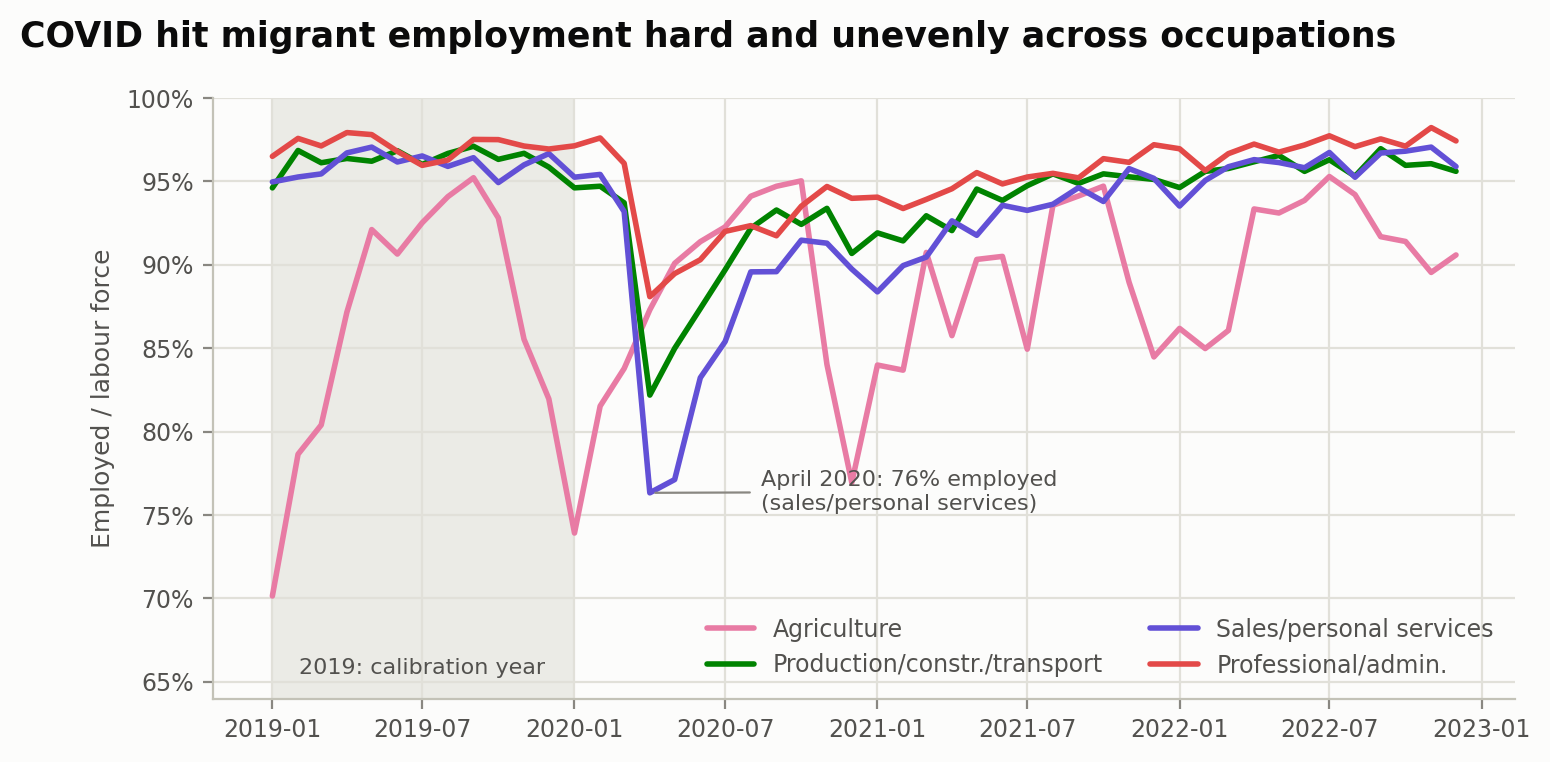
\includegraphics[width=0.85\linewidth]{B1_cps_employment.png}
\caption{\textbf{US employment by occupation.} Monthly employment rate of Mexican-origin workers aged 18--64 by occupation of current or last job, CPS, 2019--2022. These rates drive migrants' monthly ability to send.}
\label{fig:cps}
\end{figure}

\begin{figure}[h]
\centering
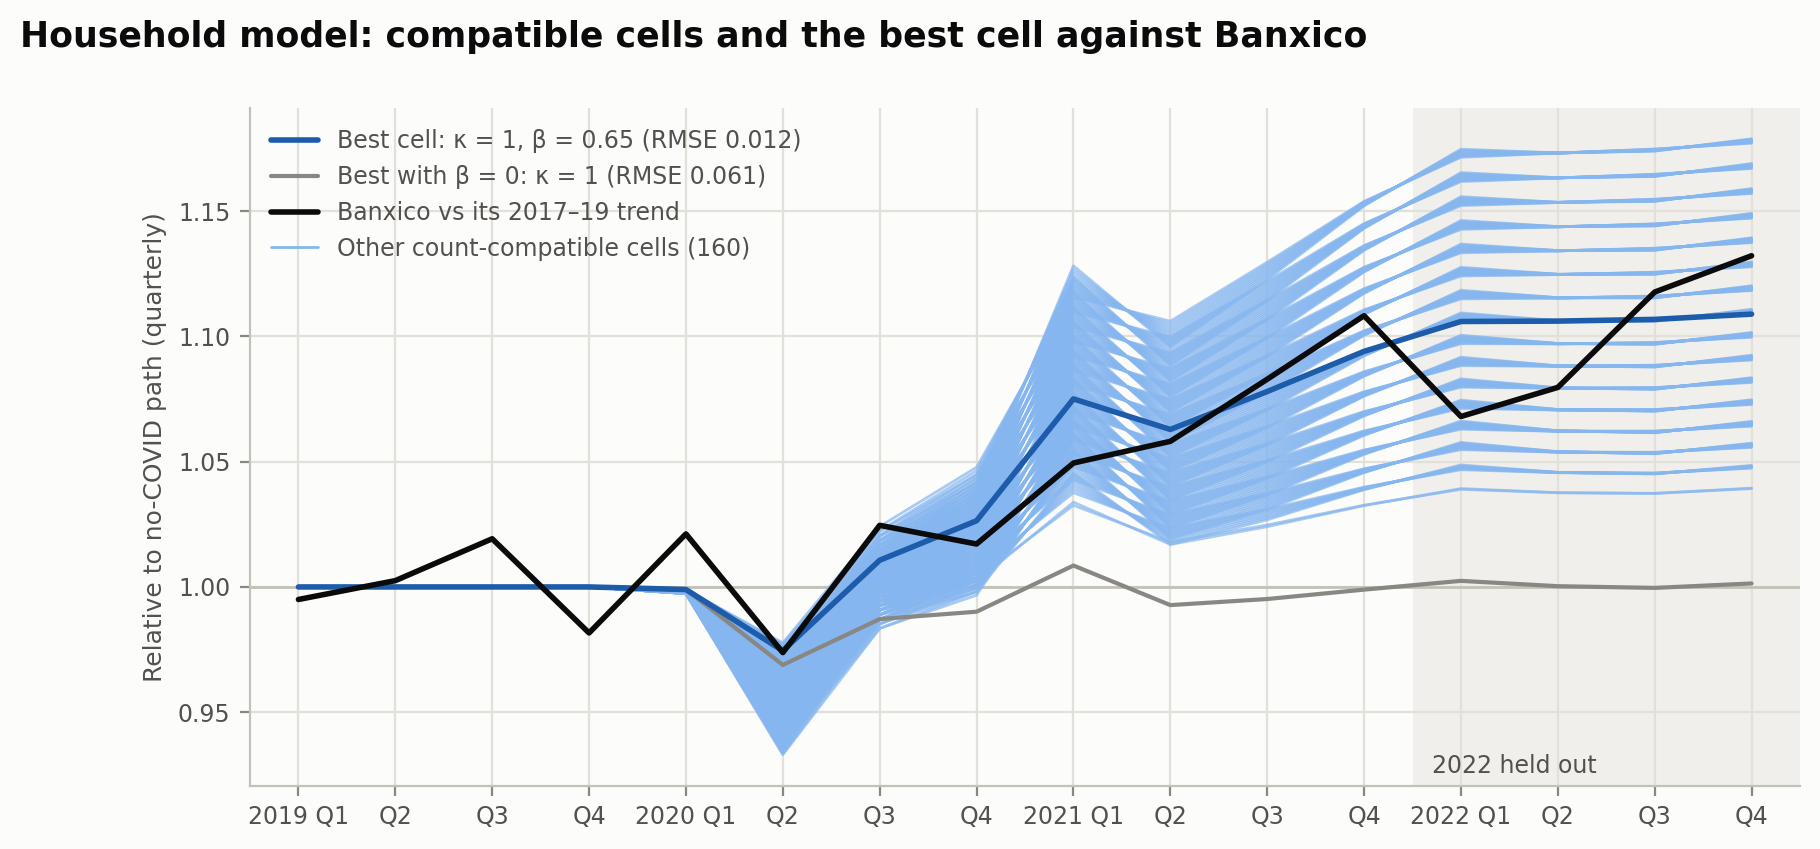
\includegraphics[width=0.92\linewidth]{S6_compatible_paths.png}
\caption{\textbf{Compatible paths.} Quarterly transfer index of all configurations within the tolerance, the best configuration and the best configuration without need, against Banco de M\'exico counts relative to trend. 2022 held out.}
\label{fig:paths}
\end{figure}

\begin{figure}[h]
\centering
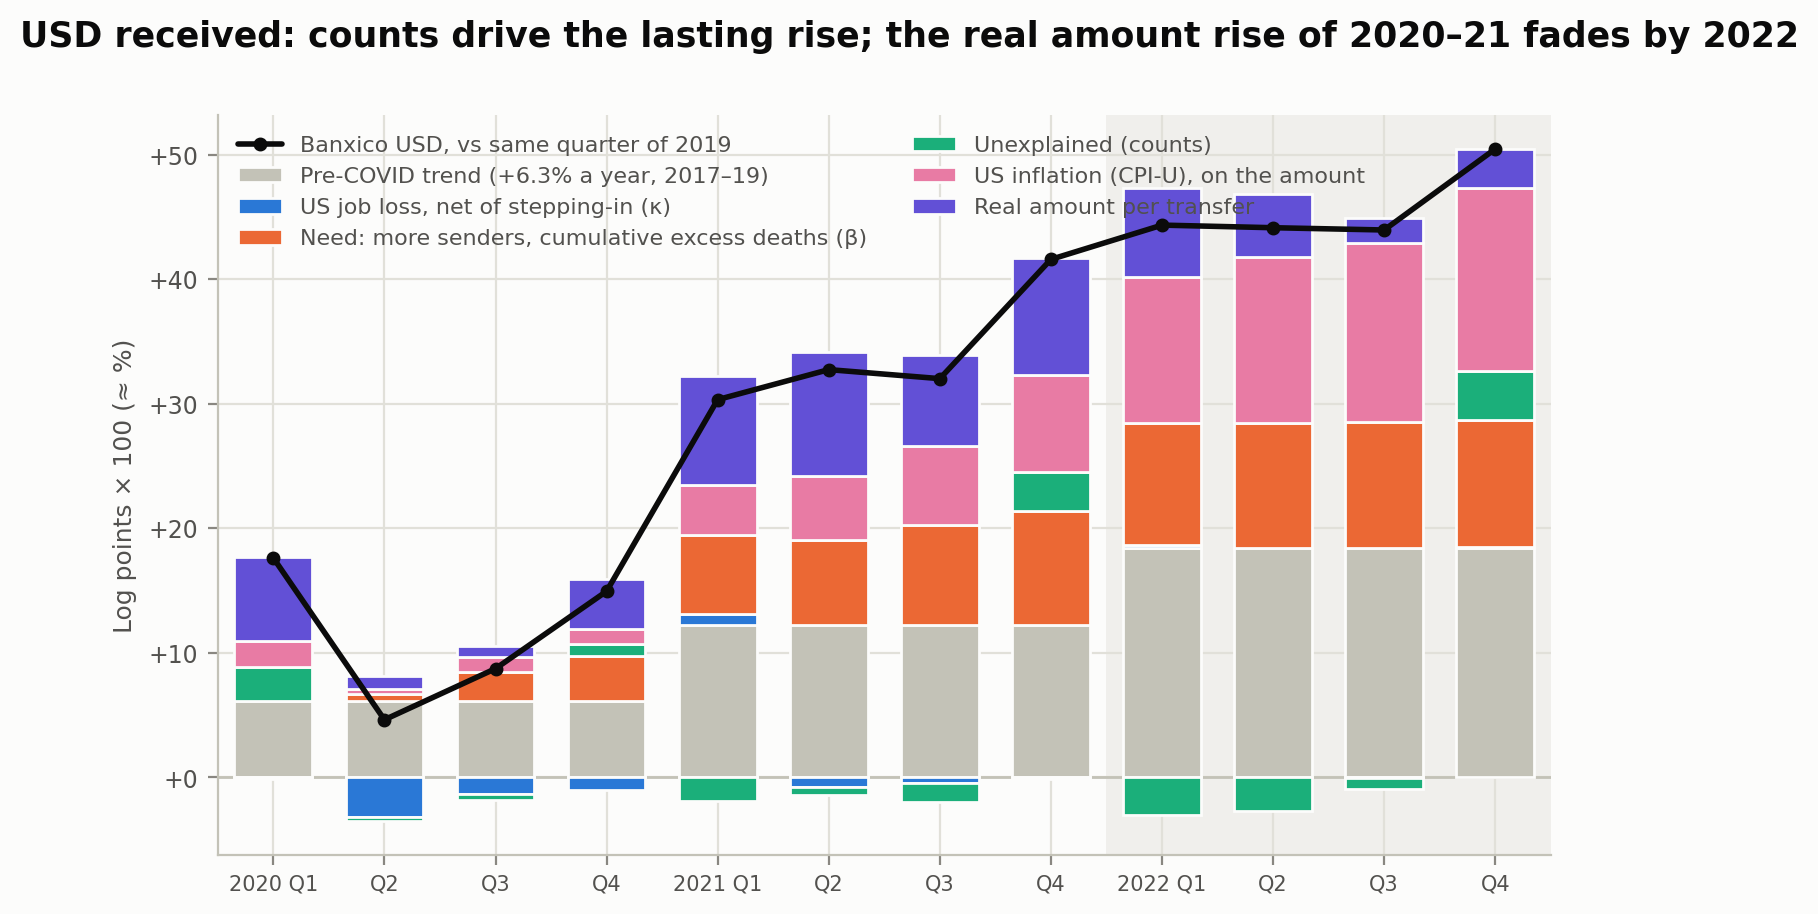
\includegraphics[width=0.92\linewidth]{S10_usd_accounting.png}
\caption{\textbf{From counts to dollars.} Banco de M\'exico remittances in US dollars relative to the same quarter of 2019 = transfer counts (decomposed as in Fig.~\ref{fig:decomp}) $\times$ average amount per transfer, split into US consumer-price inflation and the real amount.}
\label{fig:usd}
\end{figure}

\end{document}
